\begin{frame}{Motivación}

    \begin{figure}[ht]
        \begin{center}
            
\includegraphics[height=1.5in]{images/caos.pdf}
        \end{center}
    \end{figure}

    \pause
    \begin{figure}[ht]
        \begin{center}
            
\includegraphics[height=1.5in]{images/horror.png}
        \end{center}
    \end{figure}
\end{frame}

\begin{frame}{Motivación}
    \begin{block}{Trabajando en grupo}
        \begin{itemize}
            \item Enviar cambios por mail, o
            \pause
            \item Enviar archivos por Discord, o
            \pause
            \item Sincronizar cambios por Google Docs.
        \end{itemize}
    \end{block}
\end{frame}

\begin{frame}{La Shell}
\begin{block}{¿Qué es?}
    \begin{itemize}
        \item Interactuamos con la computadora a través de una interfaz.
        \pause
        \item Puede ser gráfica (GUI).
            \begin{figure}
            \begin{minipage}{.5\textwidth}
              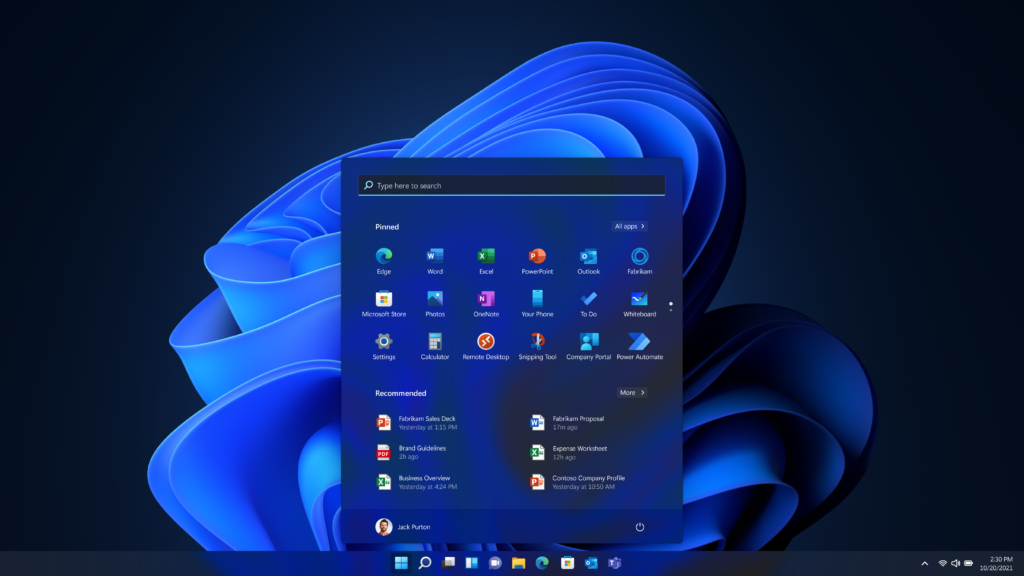
\includegraphics[width=.8\linewidth]{images/windows-gui.png}
            \end{minipage}%
            \begin{minipage}{.5\textwidth}
              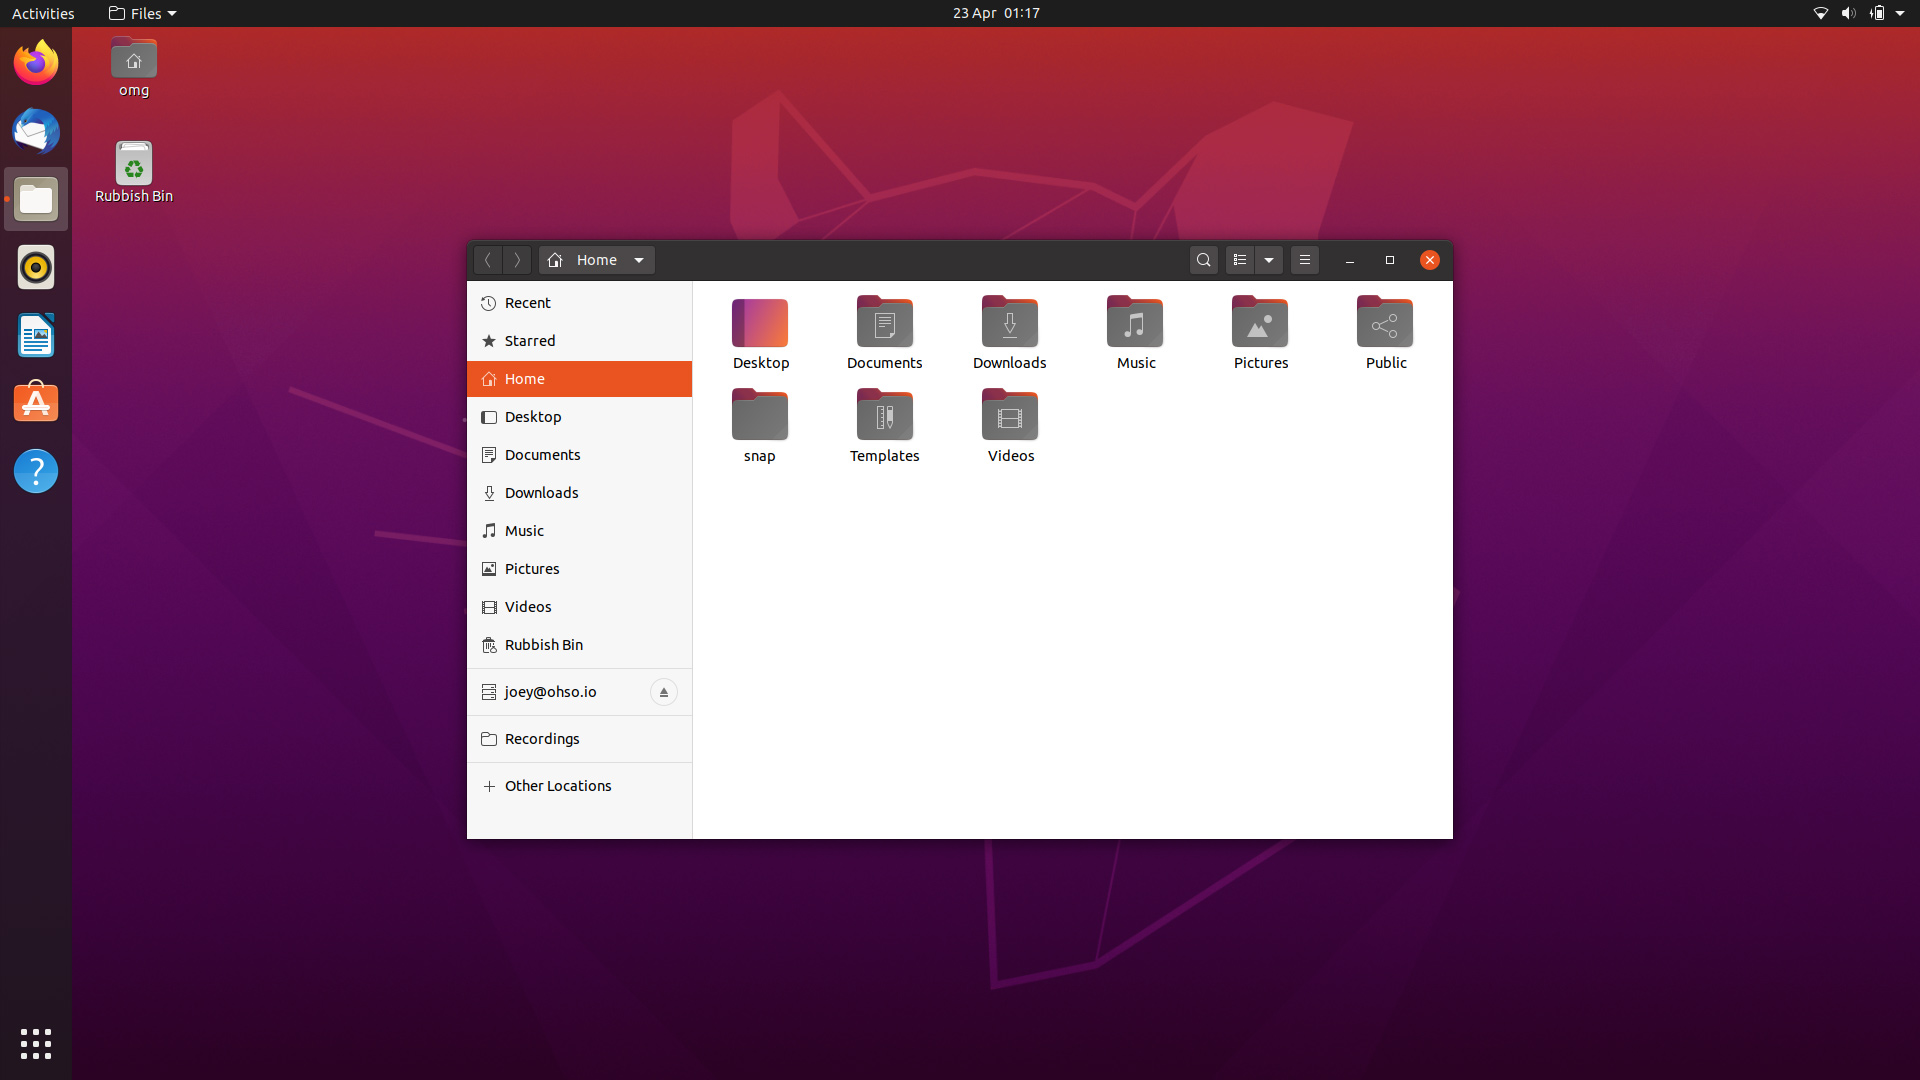
\includegraphics[width=.8\linewidth]{images/ubuntu-gui.jpg}
            \end{minipage}
            \end{figure}
        \pause
        \item O de línea de comando (CLI).
    \end{itemize}
\end{block}

\end{frame}

\begin{frame}{La Shell (2)}
    \begin{block}{¿Qué es? (2)}
        \begin{itemize}
                \item Bash AKA \textit{Bourne-Again SHell}
            \pause
            \item Para abrir un \textit{shell prompt,} necesitamos una terminal.
            \pause
        \end{itemize}
    \begin{centering}
    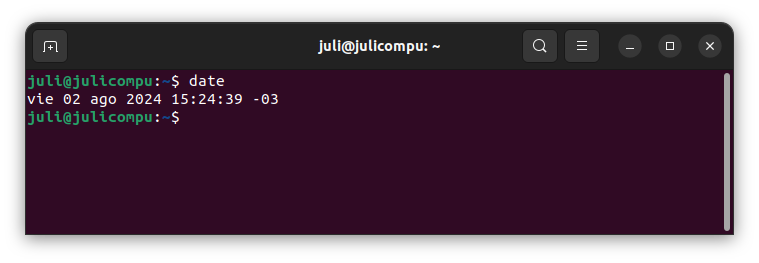
\includegraphics[height=1.5in]{images/bash-1.png}        
    \end{centering}
    \end{block}

\end{frame}

\begin{frame}{La Shell (3)}
\begin{block}{Navegando la Shell}
        \vspace{-0.3cm}
        \centering
        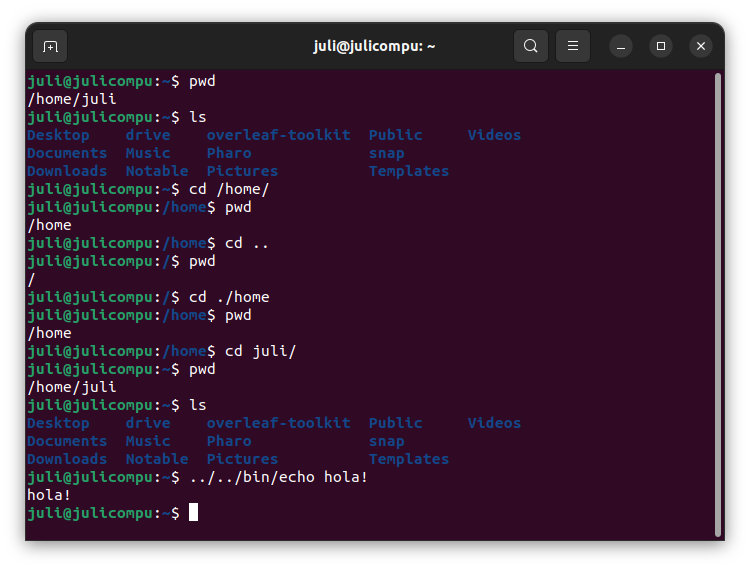
\includegraphics[width=4in]{images/bash-3.png}
\end{block}
\end{frame}
